\documentclass[10pt]{beamer}

  % Math Packages
  \usepackage{amsmath}
  \usepackage{amsthm}
  \usepackage{mathtools}

  % Graphics Packages
  \usepackage{graphicx}
  \graphicspath{ {../_static/images/} }
  \usepackage{pgf}
  \usepackage[export]{adjustbox}

  % Code listings
  \usepackage{listings}
  \lstset{language=Python, basicstyle=\footnotesize}

  % Misc packages
  \usepackage{hyperref}
  \hypersetup{colorlinks=true,linkcolor=,urlcolor=blue}

  % Colors
  \definecolor{myblue}{RGB}{25,98,148}
  \definecolor{mygray}{RGB}{66,66,66}

  % Theme Settings
  \usetheme[subsectionpage=progressbar]{metropolis}

  % \setbeamercolor{normal text}{fg=mygray}
  % \setbeamercolor{alerted text}{fg=myblue}
  % \setbeamercolor{title text}{fg=mygray}
  % \setbeamercolor{title separator}{fg=myblue}
  % \setbeamercolor{progress bar}{fg=myblue}
  % \setbeamercolor{frametitle}{bg=myblue}

\title{Writing Python Packages}

\date[]{\today}

\begin{document}

% Title Slide
\begin{frame}
  \titlepage
\end{frame}

% ------------------------- %
% Motivation
% ------------------------- %
\section{``Good'' research}

  \begin{frame} \frametitle{What does good research look like?}

    Good research is:

    \begin{enumerate}
      \item<2-> Accurate: Mitigate potential errors
      \item<3-> Collaborative: Two brains are better than one
      \item<4-> Constructive: Engages with previous research
      \item<5-> Foundational: Provides foundation for others to engage with your work
    \end{enumerate}

    \vspace{0.25cm}

    \textbf{How can we make sure our research reflects these values?}

  \end{frame}

  \begin{frame} \frametitle{Themes of this weekend}

    This weekend we will cover tools that help us achieve these values:

    \begin{itemize}
      \item Code style, code modularity, and package development
      \item Unit and integration testing
      \item Model testing
    \end{itemize}

  \end{frame}


% ------------------------- %
% Code structure and style
% ------------------------- %
\section{Code structure and style}

  \begin{frame} \frametitle{Stylistic Python code}

    \textbf{Coding is a form of communication\dots}

    \vspace{0.5cm}

    \begin{quote}
      Always code as if the guy who ends up maintaining your code will be a violent psychopath who
      knows where you live. Code for readability. --- John Woods
    \end{quote}

    \vspace{0.2cm}

    \begin{quote}
      Measuring programming progress by lines of code is like measuring aircraft building progress
      by weight --- Bill Gates
    \end{quote}

  \end{frame}

  \begin{frame} \frametitle{``Non-negotiable'' stylistic rules}

    These are rules I feel (maybe overly) strongly about,

    \begin{itemize}
      \item A space after EVERY comma... Except when trailing --- \texttt{foo = (0,)}
      \item Avoid wildcard imports (i.e. \texttt{from <module> import *})
      \item Four spaces for block indentation... No more, no less.
      \item Limit lines of code to roughly 80 characters
      \item Try to organize code into logical blocks
      \item No space before or after a colon
    \end{itemize}

  \end{frame}

  \begin{frame} \frametitle{Stylistic choices}

    I feel less strongly about some of these rules, but I find that they improve readability for me

    \begin{itemize}
      \item Two lines before and after a function definition
      \item Don't repeat yourself (DRY)
      \item Don't align your \texttt{=}
    \end{itemize}

  \end{frame}

  \begin{frame}[fragile] \frametitle{Examples of good code}

    {\small
    \begin{lstlisting}{GoodCode}

    import numpy as np
    from scipy.linalg import lstsq


    # Create data
    y = np.array([1.0, 4.0, 3.0, 2.0])
    x = np.array([
        [1.0, 0.5],
        [1.0, 2.0],
        [1.0, 1.5],
        [1.0, 1.0]
    ])

    # Find coefficients
    coeffs, resid, _, _ = lstsq(x, y)

    \end{lstlisting}
    }

  \end{frame}

  \begin{frame}[fragile] \frametitle{Examples of bad code}

    {\small
    \begin{lstlisting}{BadCode}

    import numpy as np
    from scipy.linalg import *
    y                = np.array([1.0, 4.0, 3.0,2.0])
    x                = np.array([[1.0,0.5],[1.0,2.0],[1.0, 1.5],[1.0, 1.0]])
    coeffs,resid,_,_ = lstsq(x,y)

    \end{lstlisting}
    }

  \end{frame}



% ------------------------- %
% Exercise
% ------------------------- %
\section{Motivational exercise!}

  \begin{frame} \frametitle{Exercise: Why write packages?}

    We are going to begin by doing some economics for two reasons:

    \begin{enumerate}
      \item We are economists --- How will these tools help us as economists?
      \item Understanding the costs associated with using low quality code helps
        motivate me to produce high quality code
    \end{enumerate}

  \end{frame}

  \begin{frame} \frametitle{Hendricks Leukhina 2017}

    Our exercise will be to replicate analysis done in \textit{How risky is college
    investment} by Lutz Hendricks and Oksana Leukhina.

    \begin{itemize}
      \item One of the key components of risk to consider when deciding to pursue college
        is ``failure to graduate'' risk
      \item To motivate the credit accumulation component of their structural model, the authors
            propose a simplified model of credit accumulation
      \item We will only replicate a small piece of their paper (Section 2)
    \end{itemize}

  \end{frame}

  \begin{frame} \frametitle{The model}

    Each individual begins as a college freshman with $n_0 = 0$ college credits

    \begin{itemize}
      \item Individual's draw an ability level $a_i \sim N(0, 1)$
      \item An individual's HS GPA is correlated with their ability level,
        $\text{GPA} = a + \varepsilon$ where $\varepsilon \sim N(0, \sigma^2)$
      \item Each year, student attempts 12 courses each worth 3 credits. They pass each
        course with a probability given by $p(a)$
      \item A student graduates if they accumulate 125 credits within 6 years and fail
        to graduate otherwise
    \end{itemize}

  \end{frame}

  \begin{frame} \frametitle{Data}

    The authors use restricted-use microdata from National Center for Education
    Statistics which has college transcript data for each student in the HS\&B survey.

    They ``calibrate'' their model through a simulated method of moments with a target
    of 10 moments:

    \begin{enumerate}
      \item The correlation between credits earned by a student the first two years of
        college
      \item The 10th/20th/\dots/80th/90th quantiles of total credits earned after two
        years
    \end{enumerate}

  \end{frame}

  \begin{frame} \frametitle{Exercise instructions}

    Everyone should clone the
    \href{https://github.com/cc7768/transcripty}{transcripty repository}

    \vspace{0.25cm}

    We will break into 4 groups and each group will receive a group number. There are a
    few constraints that groups should satisfy:

    \begin{itemize}
      \item The person who is ``driving'' should not have been the ``driver'' in the
        previous session
      \item The people who ``drove'' last time should separate themselves amongst the
        groups
      \item The groups should roughly be the same size
    \end{itemize}

  \end{frame}

  \begin{frame} \frametitle{Exercise}

    See \href{https://github.com/nyupredocs/modularizationandtesting/blob/master/Projects/Project_1_HendricksLeukhina.md}{Project 1}

    \vspace{0.25cm}

    We will work on this for 30-45 mins

  \end{frame}

  \begin{frame} \frametitle{Debrief}

    \textbf{How did you find the exercise?}

    \vspace{0.25cm}

    \textbf{Which components of code were helpful?}

    \vspace{0.25cm}

    \textbf{What slowed you down?}

  \end{frame}



% ------------------------- %
% Package development
% ------------------------- %
\section{Package development}

  \begin{frame} \frametitle{Example package: pyblp}

    \begin{center}
      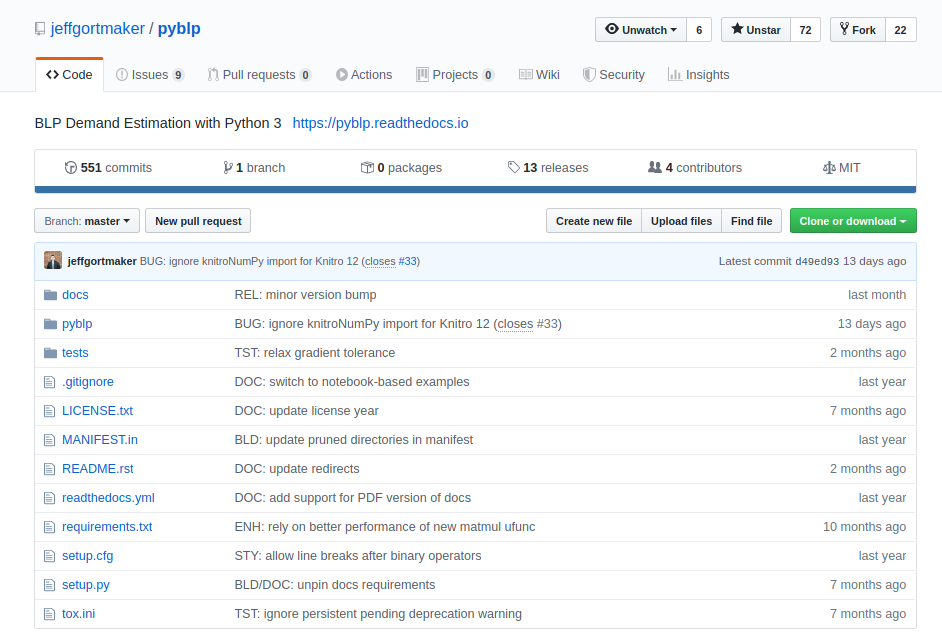
\includegraphics[width=\textwidth]{pyblp_gh_snapshot.png}
    \end{center}

    % Note the beautiful commit message conventions that Jeff uses. See
    % https://www.conventionalcommits.org/en/v1.0.0/
    % for more information and examples

  \end{frame}

  \begin{frame} \frametitle{Package structure}

    {\footnotesize
    Most Python packages share a similar structure:

    \begin{itemize}
      \item \texttt{docs}: This folder contains the files that help generate the documentation.
      \item \texttt{<package\_name>}: This folder contains the package source code and is what will
        be loaded by Python when \texttt{import <package\_name>} is called.
      \item \texttt{tests}: This folder contains the unit and integration tests
      \item \texttt{README.\{md,rst,txt\}}: This is a file that introduces the package and will be
        rendered on the github landing page.
      \item \texttt{LICENSE.txt}: You should not use a package that is not licensed because
        (according to people who know more about the law than I do) your work is under an
        exclusive copyright by default. Useful to read through \url{https://choosealicense.com}
        to learn a bit more about each license. I tend to prefer relatively permissive Apache/BSD/MIT
        licenses as opposed to copyleft licenses like GPL.
      \item Various files used to build and maintain the package. These files include
        \texttt{setup.py}, \texttt{readthedocs.yml}, \texttt{requirements.txt}, etc\dots
    \end{itemize}

    }

  \end{frame}

  \subsection{Package source code}

  \begin{frame} \frametitle{Package source code: structure}

    The package source code is organized into a collection of files and folders. We will
    refer to the folders within the package as ``sub-packages''\footnote{
    Some people get technical and refer to the elements inside of a package as modules,
    sub-modules, and sub-packages, but we're going to try and avoid these details for
    now\dots See
    \href{
    https://stackoverflow.com/questions/7948494/whats-the-difference-between-a-python-module-and-a-python-package
    }{this SO question} if you'd like to know more of the details}.

    \vspace{0.25cm}

    In \texttt{pyblp} there is a class called \texttt{SimulationMarket} in
    \texttt{pyblp/markets/simulation\_market.py}.

    \vspace{0.25cm}

    There are two ways to access this class in your Python code\dots

  \end{frame}

  \begin{frame}[fragile] \frametitle{Package source code: structure}

    First, we could do:

    \vspace{0.5cm}

    \begin{lstlisting}
    import pyblp.markets  # We could create an alias here!

    pyblp.markets.SimulationMarket(args...)
    \end{lstlisting}

  \end{frame}

  \begin{frame}[fragile] \frametitle{Package source code: structure}

    or, we could do:

    \vspace{0.5cm}

    \begin{lstlisting}
    from pyblp.markets import SimulationMarket

    SimulationMarket(args...)
    \end{lstlisting}

  \end{frame}

  \begin{frame} \frametitle{Package source code: \texttt{\_\_init\_\_.py}}

    Your Python package should have an \texttt{\_\_init\_\_.py} file within the main
    source code directory and within each sub-package.

    \vspace{0.25cm}

    This file used to be required in order to identify a directory as a package, but, as
    of Python 3.3, it is no longer a requirement.

    \vspace{0.25cm}

    However, we think it is still a good idea to include this file because it will be run
    whenever the package is imported and can be a good place to initialize relevant
    features or expose particular methods.\footnote{Can find more details in
    \href{http://python-notes.curiousefficiency.org/en/latest/python_concepts/import_traps.html}{this blogpost}
    }

  \end{frame}

  \begin{frame} \frametitle{Package source code: setuptools}

    \onslide<1->{To make your package installable, you need to create a \texttt{setup.py} file which
    uses \href{https://setuptools.readthedocs.io/en/latest/index.html}{the setuptools package}}

    \vspace{0.25cm}

    \onslide<2->{After creating a \texttt{setup.py} file, the package can be installed with
    \texttt{python setup.py install}}

    \vspace{0.25cm}

    \onslide<3->{What's in a \texttt{setup.py} file? Only \texttt{name}, \texttt{version}, and
    \texttt{packages} are required  arguments to \texttt{setup}, but it's useful to add
    include many others}

  \end{frame}

  \subsection{Documentation}

  \begin{frame} \frametitle{Documentation: writing docstrings}

    Documentation is your chance to provide your users (including yourself!) with instructions
    on what each function does and how it should be used.

    \vspace{0.25cm}

    The vast majority of functions should have a doc string.

    \vspace{0.25cm}

    I like to follow the
    \href{https://numpydoc.readthedocs.io/en/latest/format.html}{numpydoc docstring guide},
    but any format you like is fine as long as you're consistent.

  \end{frame}

  \begin{frame}[fragile] \frametitle{Documentation: numpydoc docstring conventions}

    \begin{lstlisting}{numpydoc}
    def myfunction(arg1, arg2):
        """
        This paragraph provides a description of the function.

        Parameters
        ----------
        arg1 : type(arg1)
            Description of arg1
        arg2 : type(arg2)
            Description of arg2

        Returns
        -------
        return_value : type(return_value)
            Description of return value

        See Also
        --------
        other_function : This is a related function
        """
        ...
    \end{lstlisting}

  \end{frame}

  \begin{frame}[fragile] \frametitle{Documentation: sphinx}

    \textbf{Step 1}: Create a folder called \texttt{docs}. Within that folder, run the
    command \texttt{sphinx-quickstart} from a terminal

    \vspace{0.25cm}

    \textbf{Step 2}: Edit \texttt{conf.py}
    \begin{itemize}
      \item Ensure that the first code in the file includes
        \begin{lstlisting}
        import os
        import sys
        sys.path.insert(0, os.path.abspath(".."))
        \end{lstlisting}
        this ensures that your packages will be found.
      \item Add relevant extensions to \texttt{extensions} variable ---
        This includes at least \texttt{sphinx.ext.autodoc} and
        \texttt{sphinx.ext.napoleon}\footnote{The napoleon extension is required for
        sphinx to understand documentation that follows the numpy or google doc
        standards. The autodoc extensions is just to simplify your life.}
    \end{itemize}

  \end{frame}

  \begin{frame} \frametitle{Documentation: sphinx}

     \textbf{Step 3}: Generate documentation from your package by running
     \texttt{sphinx-apidoc -o source/  ../<package\_name>} in a terminal in
     the \texttt{docs} directory --- We could also do this step manually for more control
     on the documentation organization

     \vspace{0.25cm}

     \textbf{Step 4}: Run \texttt{make html} in a terminal from the \texttt{docs}
     directory

     \vspace{0.25cm}

     \textbf{Step 5}: Open \texttt{\_build/html/index.html} in a browser and review the
     (excruciatingly ugly) docs that were generated! Clicking on \textit{Module Index}
     will take you to a page which has the documentation for all of your functions!

  \end{frame}

  \begin{frame} \frametitle{Documentation: sphinx}

    The first step to making the documentation slightly less ugly is to edit the
    \texttt{index.rst} file. It helps to add an introduction to your package at the top
    of the page.

    \vspace{0.25cm}

    You can (and should) also write some instructions for how users could use your
    package\footnote{\texttt{pyblp} has an exceptionally good documentation page\dots
    You should mimic the level of detail included.}.

  \end{frame}

  \begin{frame} \frametitle{Documentation: Read the Docs}

    \textit{Read the Docs}\footnote{Many of the sites on their page can also be accessed with
    \href{https://www.urbandictionary.com/define.php?term=RTFD}{https://rtfd.org}} is a
    site that hosts documentation (and, more importantly, automates documentation
    updates).

    \vspace{0.25cm}

    Many open source projects (especially in the Python world) use \textit{Read the Docs} to host
    their documentation because of its ease of use and flexibility

  \end{frame}

  \begin{frame} \frametitle{Documentation: Read the Docs}

    \textbf{Step 1}: Create an account (I log in with my github account)

    \vspace{0.25cm}

    \textbf{Step 2}: Create a \texttt{readthedocs.yml} file for setting project
    specific configuration --- You won't always need this but it doesn't hurt to have a
    placeholder

    \vspace{0.25cm}

    \textbf{Step 3}: Import your package using their online tool --- Doing this takes
    care of the webhook that will automatically rebuild your docs whenever a push happens
    to the desired branch

  \end{frame}

  \subsection{Publishing Python packages}

  \begin{frame} \frametitle{Python Package Index}

    The \textit{Python Package Index} (PyPI) is ``a repository of software for the Python programming
    language.'' There are over 200,000 projects currently on PyPI

    \vspace{0.3cm}

    Any package on PyPI should be able to be installed with pip\footnote{pip is a recursive
    acronym and stands for \textit{pip installs packages}} by running
    \texttt{pip install <package\_name>}

  \end{frame}

  \begin{frame} \frametitle{Publish package on PyPI}

    \textbf{Step 1}: Install the \texttt{twine} package with \texttt{pip install twine}

    \vspace{0.25cm}

    \textbf{Step 2}: Register on \href{https://pypi.org/account/register/}{PyPI} (and
    \href{https://test.pypi.org/account/register/}{test PyPI}) --- Today we'll upload our
    packages to the test index, but you would typically use the main one

    \vspace{0.25cm}

    \textbf{Step 3}: Create the \textit{distribution package} which is essentially just
    a zipped file with your code using \texttt{python setup.py sdist bdist\_wheel}

  \end{frame}

  \begin{frame} \frametitle{Publish package on PyPI}

    \textbf{Step 4}: Check that the long description will correctly render using
    \texttt{twine check dist/*}

    \vspace{0.25cm}

    \textbf{Optional}: You can create a keyring so that you won't have to type your
    username and password each time you upload a package --- We won't do it today, but
    see the \href{https://github.com/pypa/twine\#keyring-support}{twine documentation}
    for details

    \vspace{0.25cm}

    \textbf{Step 5}: Upload to \texttt{test.pypi.org} using
    \texttt{twine upload --repository-url https://test.pypi.org/legacy dist/*} --- If
    you were uploading to main PyPI, you could simply leave out the
    \texttt{-repository-url} argument

  \end{frame}


% --------------------------------- %
% Exercise: Write your own package
% --------------------------------- %
\section{Exercise: Writing your own package}

\begin{frame} \frametitle{Exercise: Writing your own package}

  Return to your groups from before. You will now be writing your own packages.

  \vspace{0.25cm}

  The instructions for this exercise can be found in
  \href{https://github.com/nyupredocs/modularizationandtesting/blob/master/Projects/Project_2_PackageBuilding.md}{Project 2}.

\end{frame}

\end{document}

